\documentclass[11pt]{article}

\usepackage{amssymb}
\usepackage{graphicx}
\usepackage{hyperref}
\usepackage{float}
\usepackage{amsmath}
\usepackage{subcaption}
\usepackage[export]{adjustbox}

\begin{document}

\title{Visualizing Baboon Foraging Patterns and Leadership Dynamics}
\author{Ian Van Buskirk}
\date{}
\maketitle

\section{Introduction}

The primary aim of this work is to uncover the leadership dynamics of a troop of baboons and more broadly why they make the decisions they do with respect to where (and potentially when) to forage. This system is not only of intrinsic scientific interest, but is a compelling model of decision making in a complex social system. Indeed, because the troop is cohesive (i.e. stays together) each decision represents a group of sophisticated primates arriving at a consensus. Hopefully, the insights this specific analysis generates can help shape broader thoughts on coarse-graining and social systems.

The dataset that supports this work has been analyzed in a number of previous studies \cite{strandburg2015shared,strandburg2017habitat,farine2017individual}. While these studies found the troop to be largely democratic in their decision making, the general literature does not offer a consensus view~\cite{tokuyama2017leadership,lee2016partially,king2011rule,stueckle2008follow,sapolsky2007primate}. How baboons make decisions about where and when to forage remains an open question.

I begin by describing the data along with a coarse-graining method I developed to aid in visualization and analysis. I then briefly describe a central finding of past work with this data, its insufficiencies, and why I feel further analysis is necessary to uncover the dynamics of interest in this system.

\section{Methods}

\subsection{Data}

This study takes as its focus the movement dynamics of a single troop of olive baboons (\textit{Papio anubis}). This troop was studied in the field at the Mpala Research Center in Kenya during the Summer of 2012 by fitting 26 out of 46 individuals in the troop with GPS collars and recording their location each second from dawn to dusk for as many days as the battery of each GPS collar would allow. Original research using this data focused on the first 14 days of the study due to GPS collars failing over the study period. Figure~\ref{fig:dayspresent} shows how long each baboon's collar stayed active along with basic data on sex and life stage.

\begin{figure}[H]
    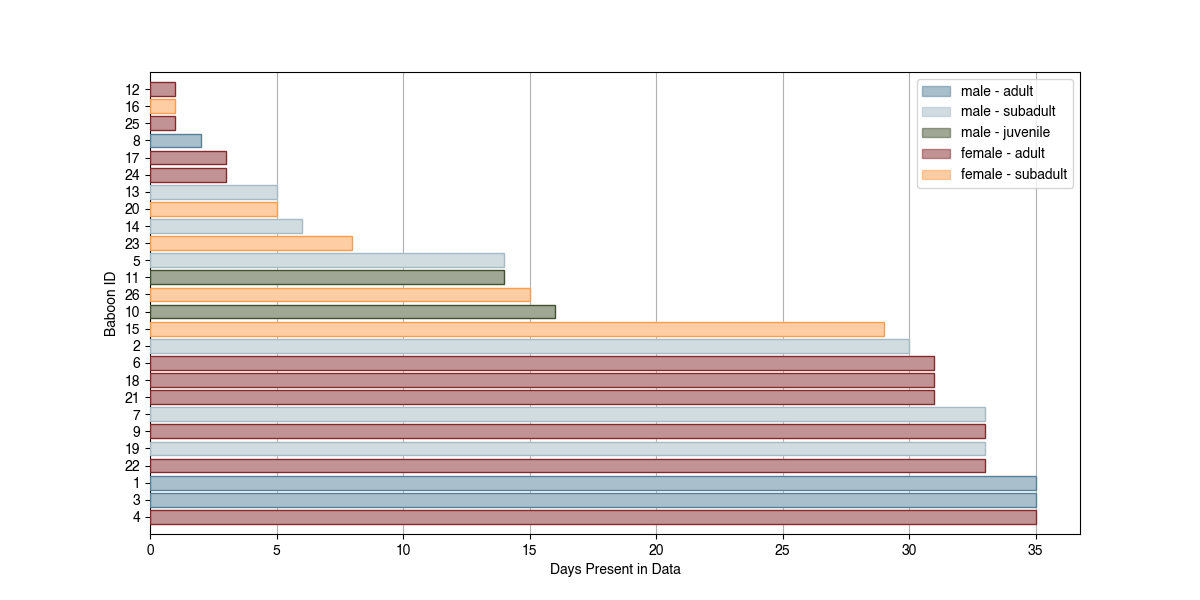
\includegraphics[width=\textwidth, valign=t]{../figures/baboon_days_present_5.png}
    \caption{The number of days each baboon appears in the dataset. Analyses must be mindful which baboons they choose to study. To select the wrong subset could mean comparing baboons with drastically different amounts of data, focusing on too small a percentage of the troop, or limiting analysis to too few days.}\label{fig:dayspresent}
\end{figure}

\newpage

Despite the collar failures, 19,206,585 positional datapoints were collected. This gives a rich reflection of troop life over the period of study and makes possible many kinds of analyses. Figure~\ref{fig:alldata} visualizes the entirety of the dataset, converted from latitude and longitude values to the xy-plane. Even here though, each trajectory (the data for a single baboon on a single day) is downsampled: only every 20th datapoint is used to trace its path. Immediately, patterns appear to push through the fuzz. To pull them out further it is clear that more sophisticated techniques than simple downsampling are necessary.

\begin{figure}[H]
    \centering
    \includegraphics[width=.75\textwidth, valign=t]{../figures/all_datapoints.png}
    \caption{All trajectories visualized at once. The GPS data from all baboons across all days is layered to get the broadest picture of troop behavior. One can see darker regions that correspond to where the troop spent more time, traveled on multiple days, or traced a particularly narrow path.}\label{fig:alldata}
\end{figure}

\subsection{Coarse-Graining}

To deal with the abundance of data this system offers I developed a custom coarse-graining scheme that enables visualization and analysis at various scales. Here, I will describe this scheme and the results of its application. I briefly discuss its role in answering questions concerning leadership dynamics in section~\ref{sec:babdiscussion}.

The coarse graining of a trajectory begins by specifying a spatial scale, $r_h$. This spatial scale defines the radius of hexagons in a hexagonal grid which is used to tesselate the xy-plane. The goal of this coarse-graining is to map the original trajectories onto this hexagonal grid so that the movement of baboons is defined discretely and with fewer datapoints.

An issue arises if one naively maps every point in the fine-grained trajectory to the center of the hexagon in which it falls: a baboon that ``mills'' on a boundary would be shown as bouncing rapidly back and forth in the coarse-grained trajectory (Fig.~\ref{fig:milling}). To avoid this issue, I introduce an event radius ($r_e$) unique to the selected spatial scale. The function of the event radius is to determine when a baboon has moved sufficiently far from its initial hexagon center for the action to qualify as a real movement at the coarser scale. Now, the original trajectory can be transformed into a sequence of events where each event is the movement of a baboon from one hexagon to another.

\begin{figure}[H]
    \centering
    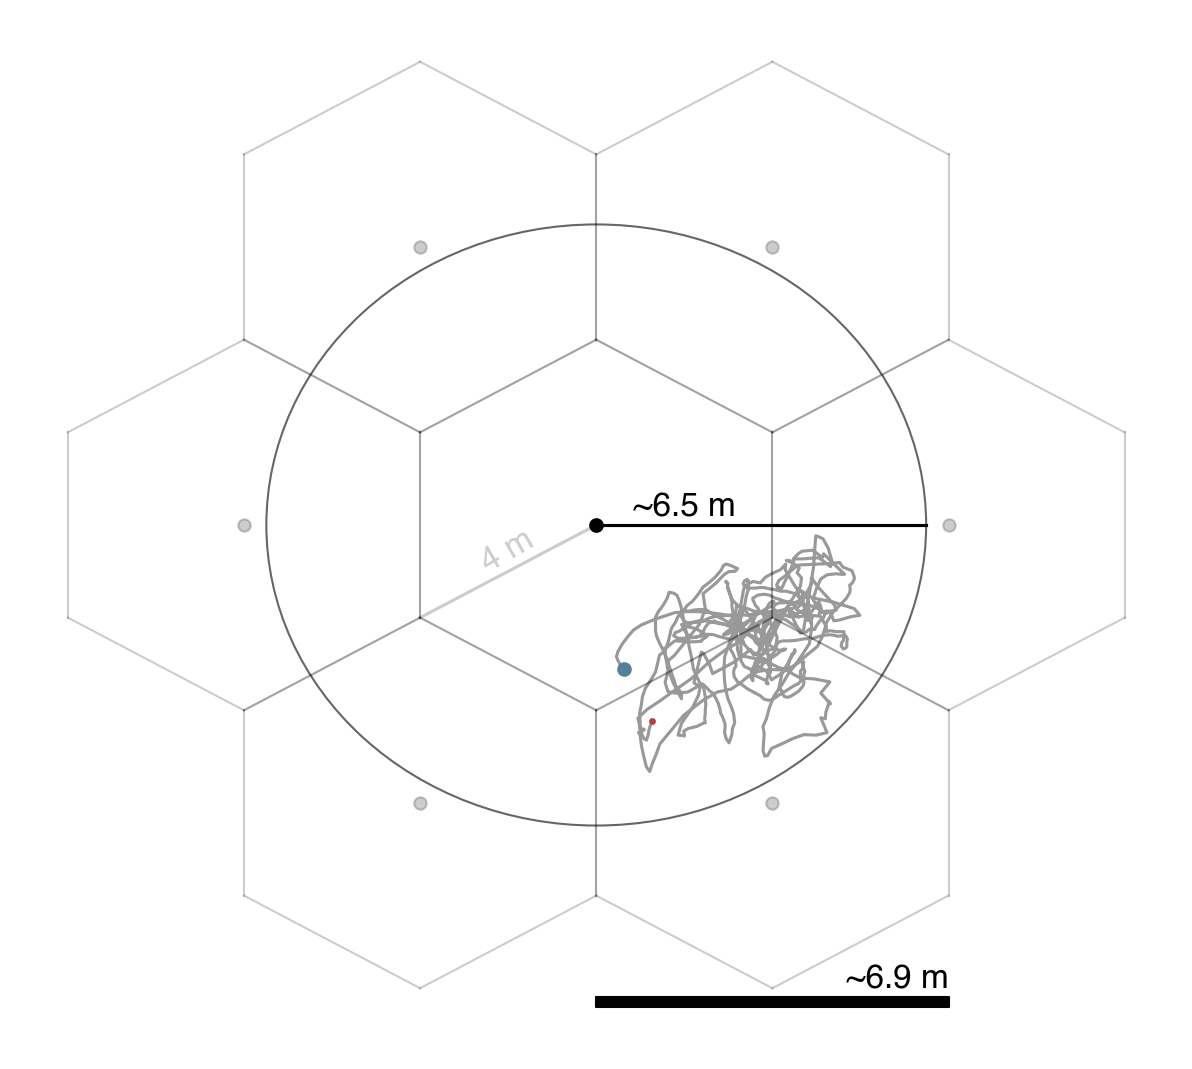
\includegraphics[width=.6\textwidth, valign=t]{../figures/milling_6.png}
    \caption{Example of a baboon milling at the intersection of three hexagons. The baboon started at the blue dot and milled for 15 minutes at which point it was found at the red dot. Although the baboon changes hexagons multiple times over this period it doesn't meaningfully move from its starting location. To account for situations like this our coarse-graining method only registers a baboon as switching hexagons if it achieves a specific distance from its hexagon center that is strictly greater than the hexagon radius. This distance is called the event radius and here it is approximately 6.5 meters (about 1.622 times the 4 meter hexagon radius). This event radius is just shy of the approximately 6.9 meters from one hexagon center to another.}\label{fig:milling}
\end{figure}

Each event has a variable duration attributable to the behavior of the baboon. However, the distances traveled should be roughly the same in every event. For this reason the event radius for a scale is chosen to minimize the variance of the distances traveled across events. This is done by randomly sampling empirical trajectories, completing the coarse-graining, computing the variance in event distances, then using a golden-section search on the window from 1.25 to 1.75 times the scale to find the event radius that minimizes variance. A piecewise function was fit to the resulting empirical estimates of event radii for purposes of smoothing and interpolation (Fig.~\ref{fig:radii}).

It is worthwhile to draw attention to one feature of the event radii estimates: once the scale reaches approximately 9 meters the event radius that minimizes variation in event distances is well modeled by a single value around 1.71 times the scale. This has a convenient interpretation. The distance between the centers of two neighboring hexagons is $r_h\sqrt{3}$. This is approximately $1.73r_h$ so our method has converged on a value which tends to drop baboons just short of the centers of the hexagons to which they transition. Or potentially, if one takes into account the distance a baboon travels in the final step crossing the event radius, as close to the center as possible. This also fits with the observation that as scale increases the event radius increases relative to the scale. When the scale is small, more distance as a fraction of the scale is covered in any step so if baboons are going to land in the centers of neighboring hexagons the event radius must be smaller (as a multiple of scale) to account for that transition (Fig.~\ref{fig:milling}).

\begin{figure}[H]
    \centering
    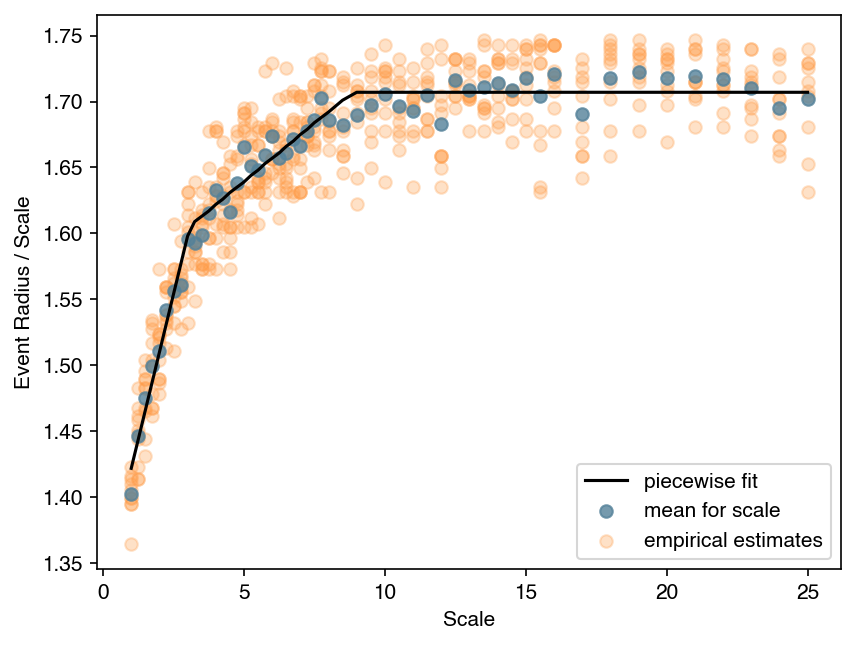
\includegraphics[width=.5\textwidth, valign=t]{../figures/radii_estimates_2.png}
    \caption{Empirical estimates for event radius as a multiple of coarse-graining scale and a piecewise fit to those estimates for various coarse-graining scales. The mean of the empirical estimates for each scale is shown as well.}\label{fig:radii}
\end{figure}

This coarse-graining provides a simple but robust way to represent the dynamical system across multiple scales. In figure~\ref{fig:cgtrajexample} I show the trajectory of one baboon on the first day of the study alongside coarse-grained trajectories using 2 and 4 meter scales. While it is clear information is lost in the coarse-graining, much is preserved. Further, whereas 43,147 datapoints are needed to trace the original trajectory only 2,276 and 992 datapoints are used to trace the 2 and 4 meter coarse-grained trajectories respectively. The appropriate scale will depend on the analysis, but any analysis can be repeated across scales to conduct sensitivity tests and see how troop behavior appears to change as one zooms out.

\begin{figure}[H]
    \centering
    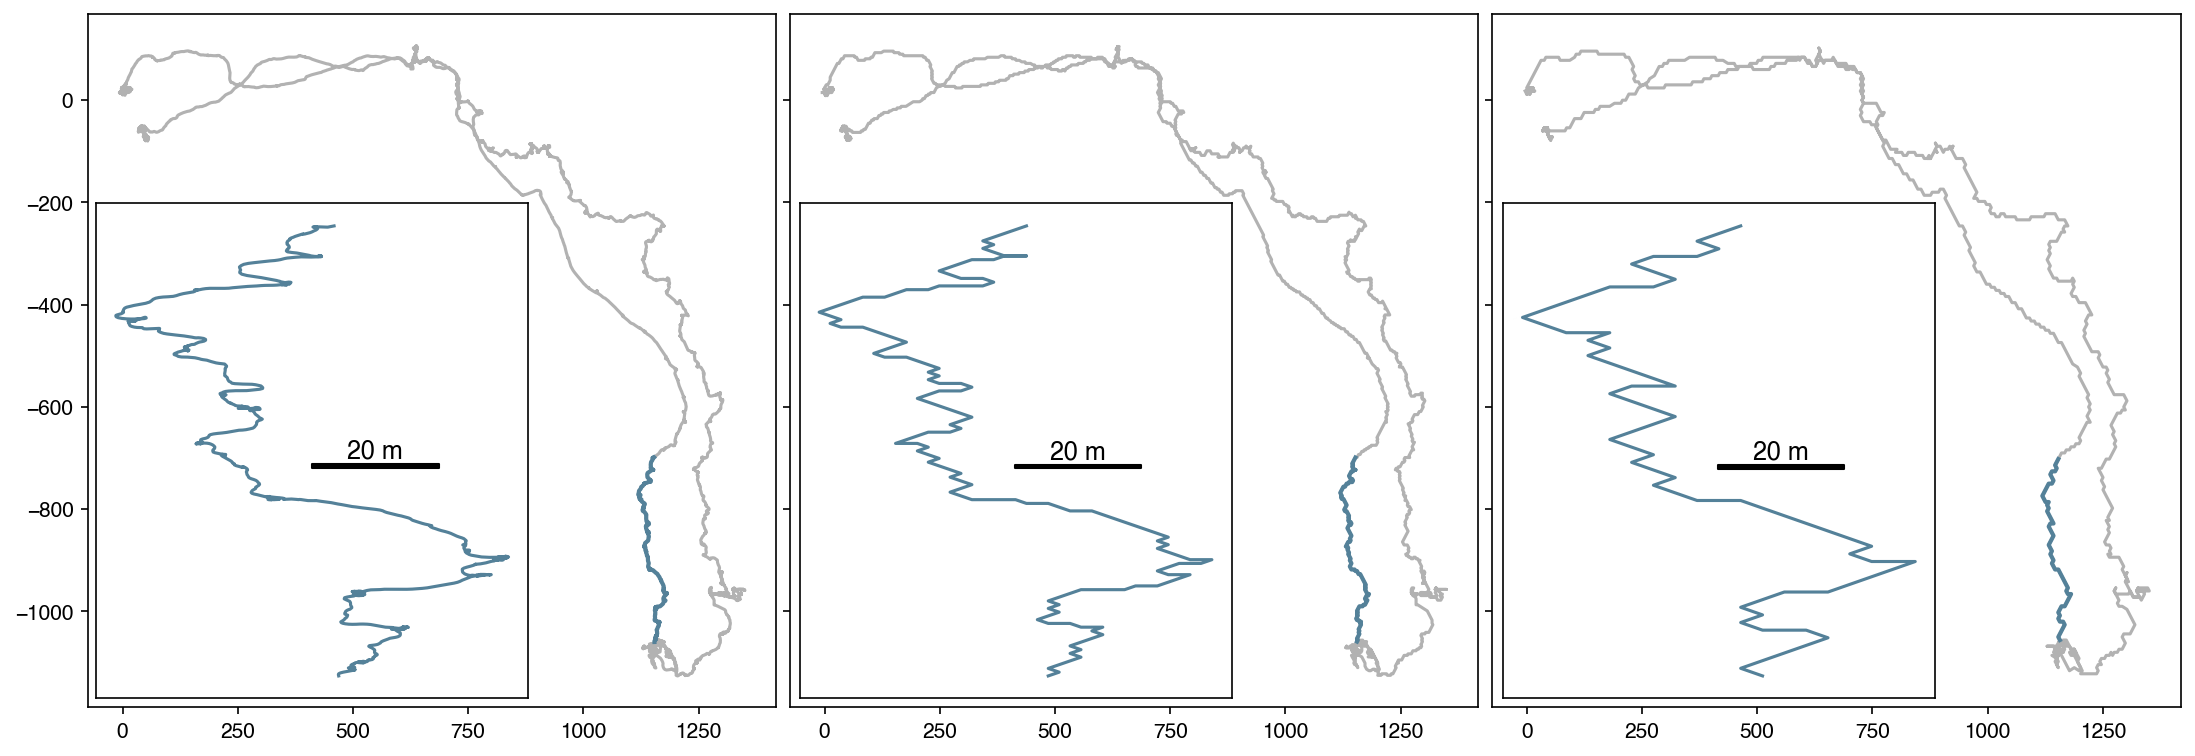
\includegraphics[width=\textwidth, valign=t]{../figures/cgtrajexample.png}
    \caption{A single trajectory from the first day of the study period (left) and two versions coarse-grained using scales of 2 meters (center) and 4 meters (right). In each figure the inset shows a zoomed in view of the blue, highlighted portion in the full trajectory.}\label{fig:cgtrajexample}
\end{figure}

I have also built a rudimentary interactive data visualization that allows one to quickly examine the system through this lens of coarse-graining. Figure~\ref{fig:interactive} shows a screenshot of the interface. One can see the hexagon that hosts each baboon as well as those hexagons that were visited some number of events before and after the focal event. This window can be made larger or smaller to show more or less of the day. One can also control the scale of the coarse-graining. Along the bottom of the interface one sees each baboon's events laid out in time. This gives an overview of when the troop is active. The job now is to translate some of the insights gained through visualization into proper analysis.

\begin{figure}[H]
    \centering
    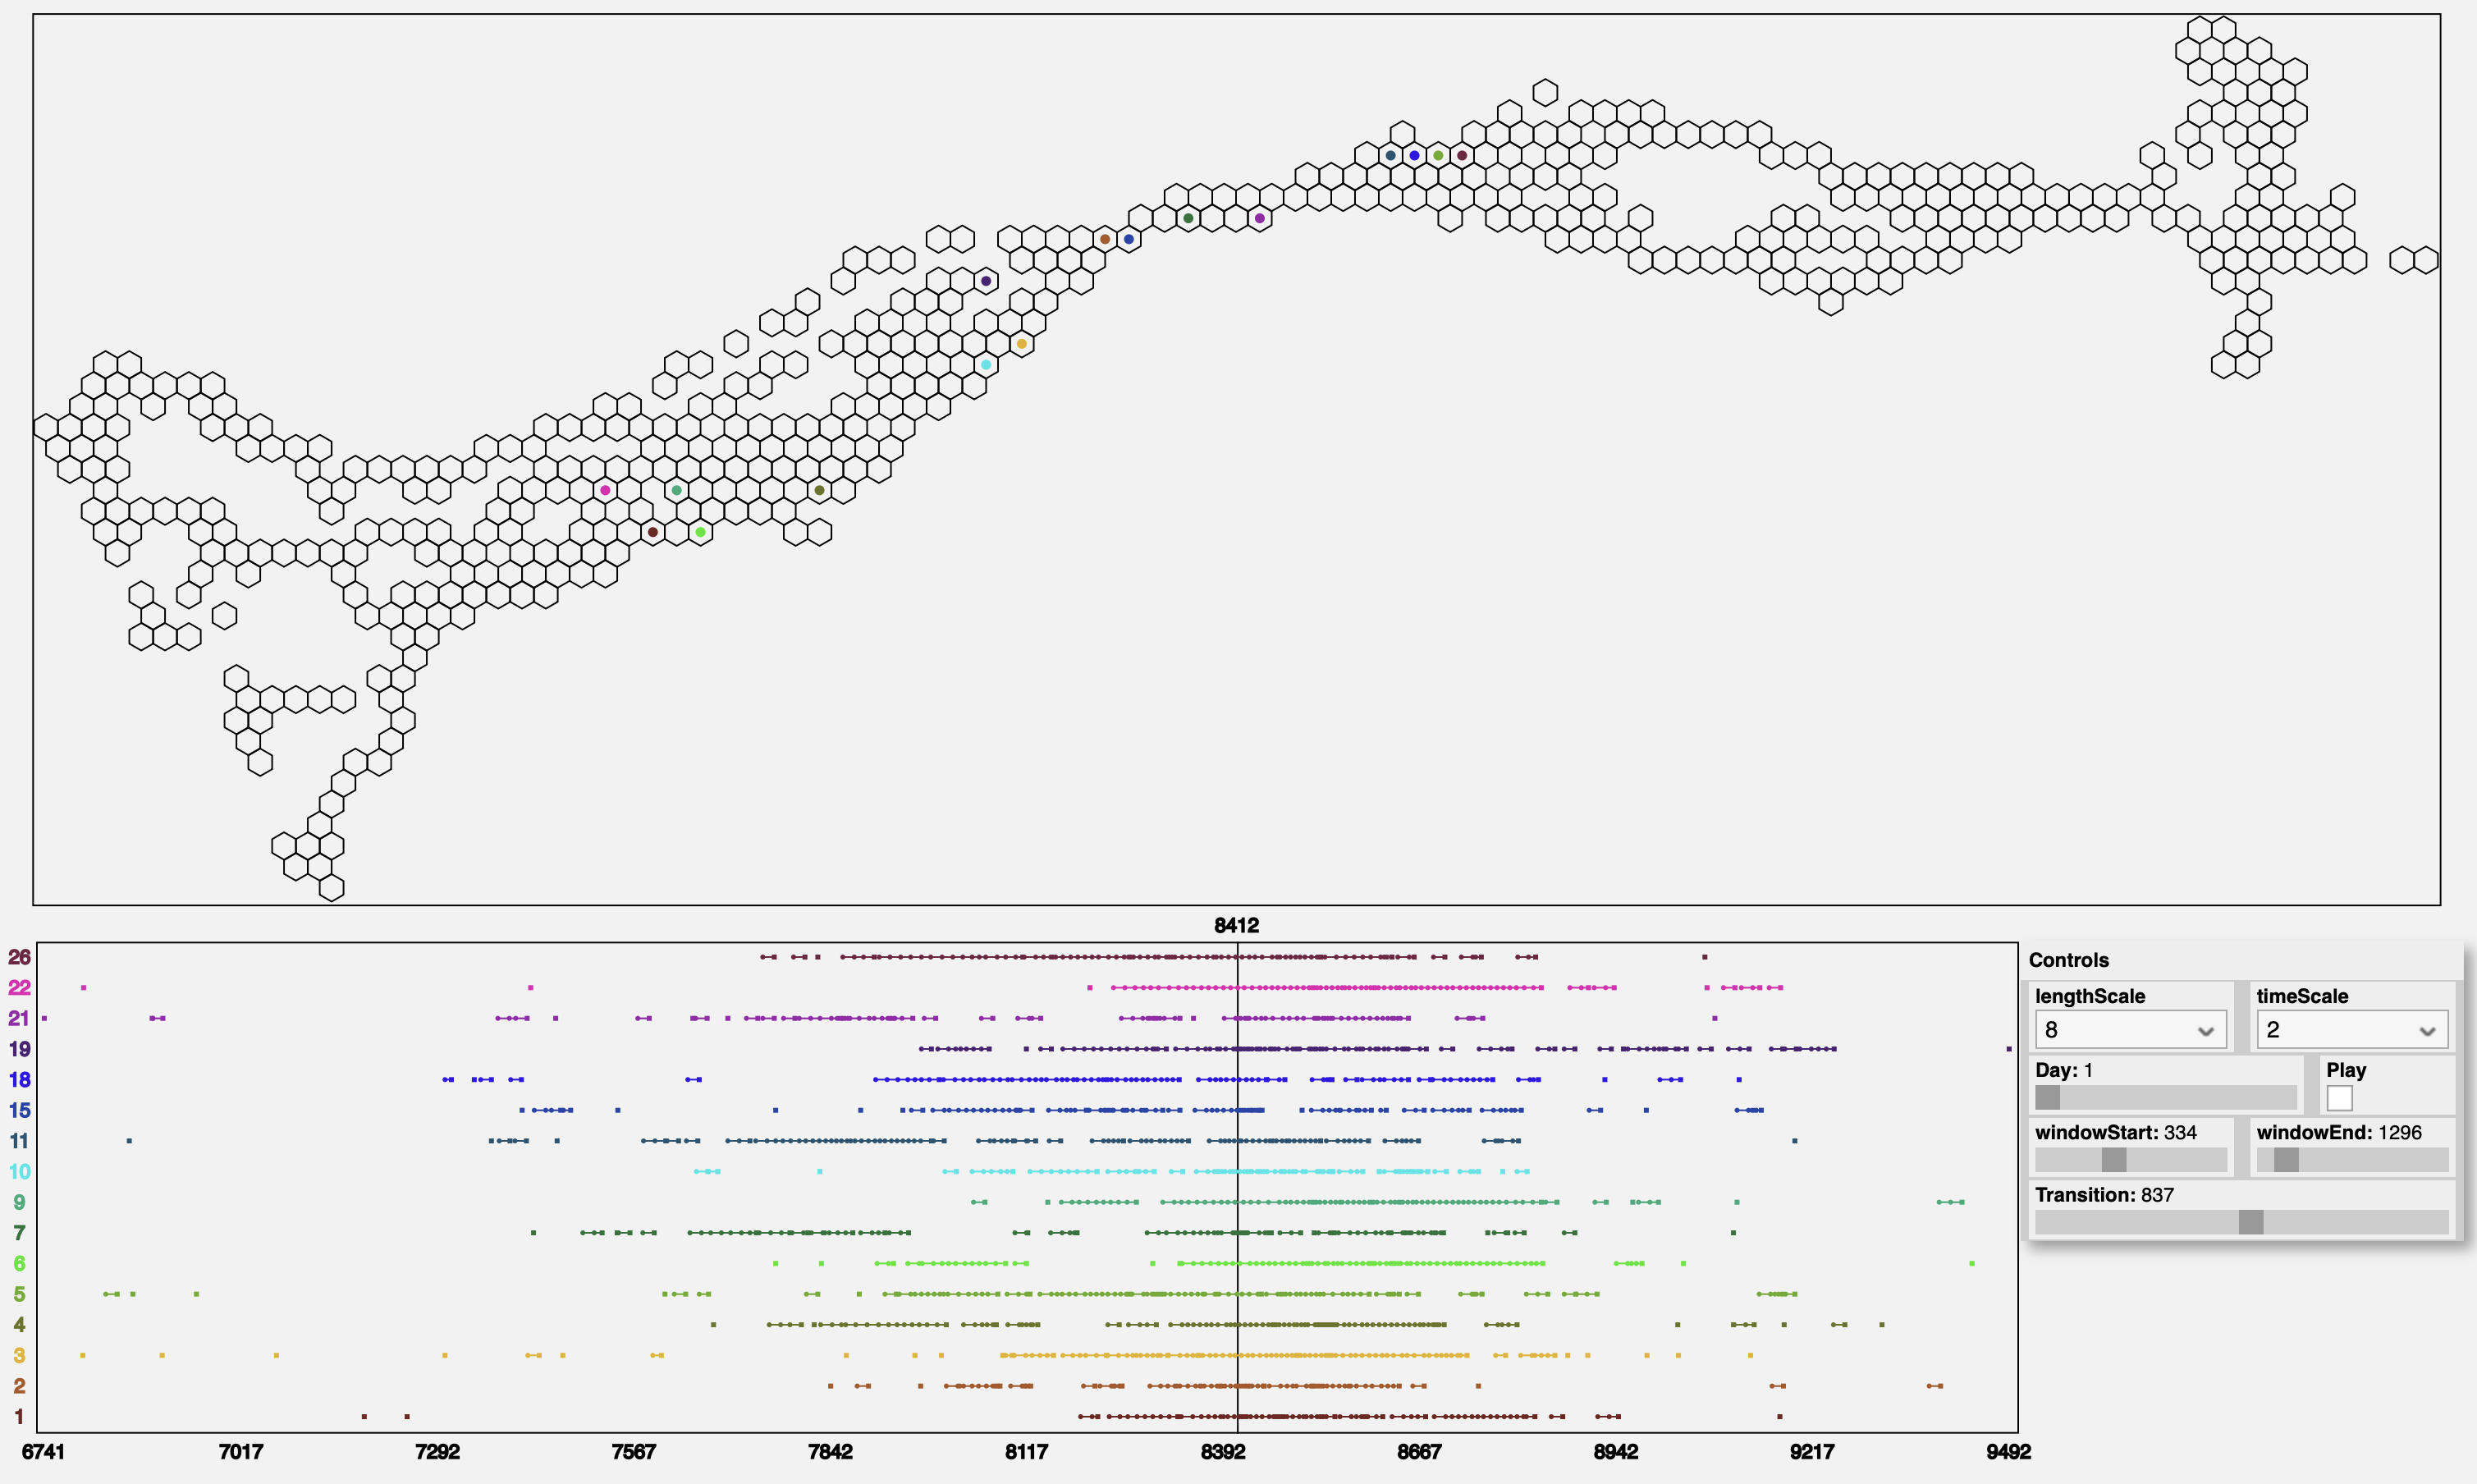
\includegraphics[width=\textwidth, valign=t]{../figures/s1.png}
    \caption{Screenshot of an interactive data visualization of coarse-grained trajectories. Each baboon's approximate location is represented with a dot alongside the hexagons in the hexagonal grid where baboons were recently or are soon to visit. This spatial representation is accompanied by a temporal one and the visualization controls. The temporal representation shows the time of each baboon's transitions over some designated window. One can control the bounds of this window, the scale of the coarse-graining, the transition in focus, and the day visualized.}\label{fig:interactive}
\end{figure}

\section{Discussion of Analysis}
\label{sec:babdiscussion}

Multiple papers have been published making use of this dataset \cite{strandburg2015shared,strandburg2017habitat,farine2017individual}. Here, we are most interested in the results based on a procedure of classifying and counting movement initiations \cite{strandburg2015shared}. For each pair of baboons, the distance between the two is computed at every point in time. Then, local minima and local maxima in that time series are found. Next, suitable sequences which start with a local minima, span a local maxmima, then conclude at another local minima are extracted for analysis. Each of these sequences is then classified as either a success or failure for the initiator. The initiator is whichever baboon moves farther during the first minima to maxima portion and the initiation is a success if the other baboon moves more than the initiator during the subsequent maxima to minima portion. Otherwise, it is a failure for the initiator \cite{strandburg2015shared}.

With these successes and failures documented, one can get an overall view of each baboon's ``Probability of being followed''~\cite{strandburg2015shared}. This was done by looking at the percentage of each baboon's initiations that were successful. Plotting this against the social dominance of each baboon formed the basis for claims of democratic decision making, a result replicated in figure~\ref{fig:dominance}.

\begin{figure}[H]
    \centering
    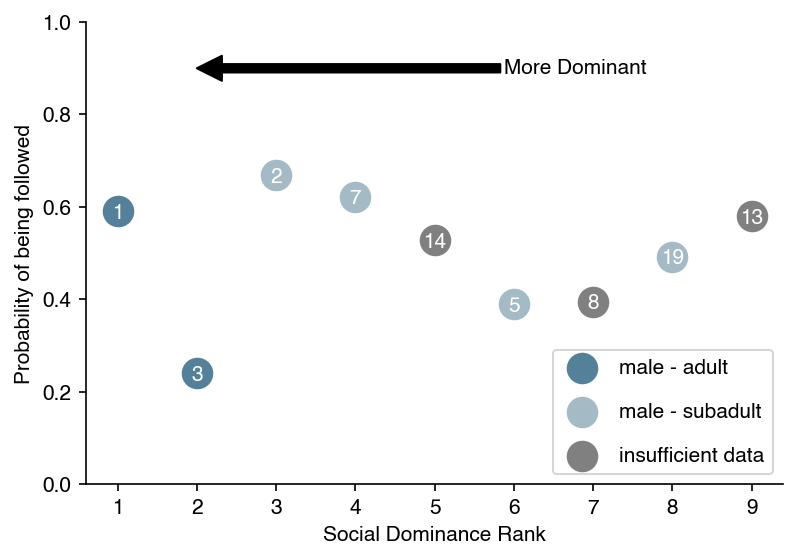
\includegraphics[height=5.5cm, valign=t]{../figures/male_dominance.png}
    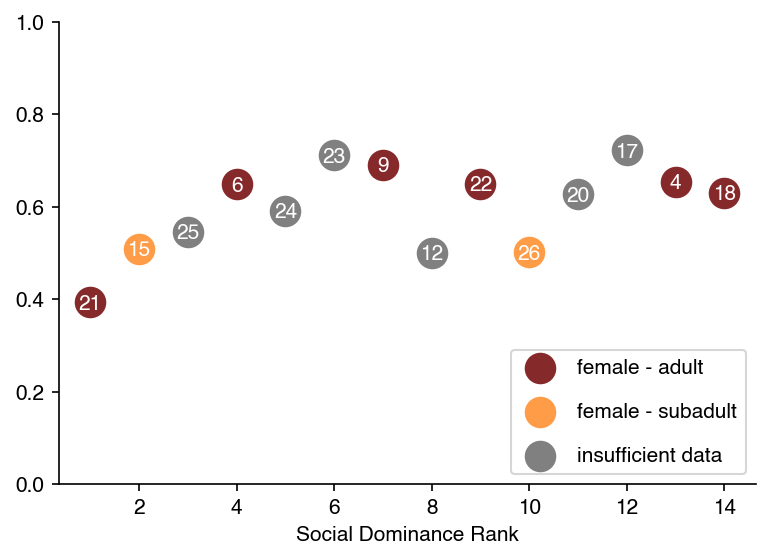
\includegraphics[height=5.5cm, valign=t]{../figures/female_dominance.png}
    \caption{A reproduction of figure S1 from Strandburg-Peshkin et al. (2015)~\cite{strandburg2015shared} based on how successful baboons are at initiating movements. Baboons represented with grey circles are those with fewer than 10 days of data. Whether these individuals are included or excluded, there is no significant relationship between social dominance rank and the probability of being followed for either male or female baboons.}\label{fig:dominance}
\end{figure}

This method of extracting and summarizing movement initiation attempts does not adequately identify moments of meaningful decision making. Although initiations are selected based on criteria that is meant to protect against false positives, too many initiations don't appear to reflect the real (lack of) influence a baboon has on where individuals or the troop ultimately decide to move. Figure~\ref{fig:initiations} supports this claim by showing where and when initiation events occur over the first 4.5 hours of the first day of the study. In total, there were 654 movement initiation events. During the first 7,500 seconds (about 2.1 hours) of this period 308 events were logged but the troop does not move from its nesting site nor do individual baboons venture far from their first logged position. Indeed, 86.4\% of these initiations are failures. During the last 4,200 seconds (about 1.2 hours) of this period 172 initiations occurred of which 91.3\% are successes. This final portion of movement sees the troop commuting: they cover more ground along a defined route in an ordered, elongated formation.

\begin{figure}[H]
    \centering
    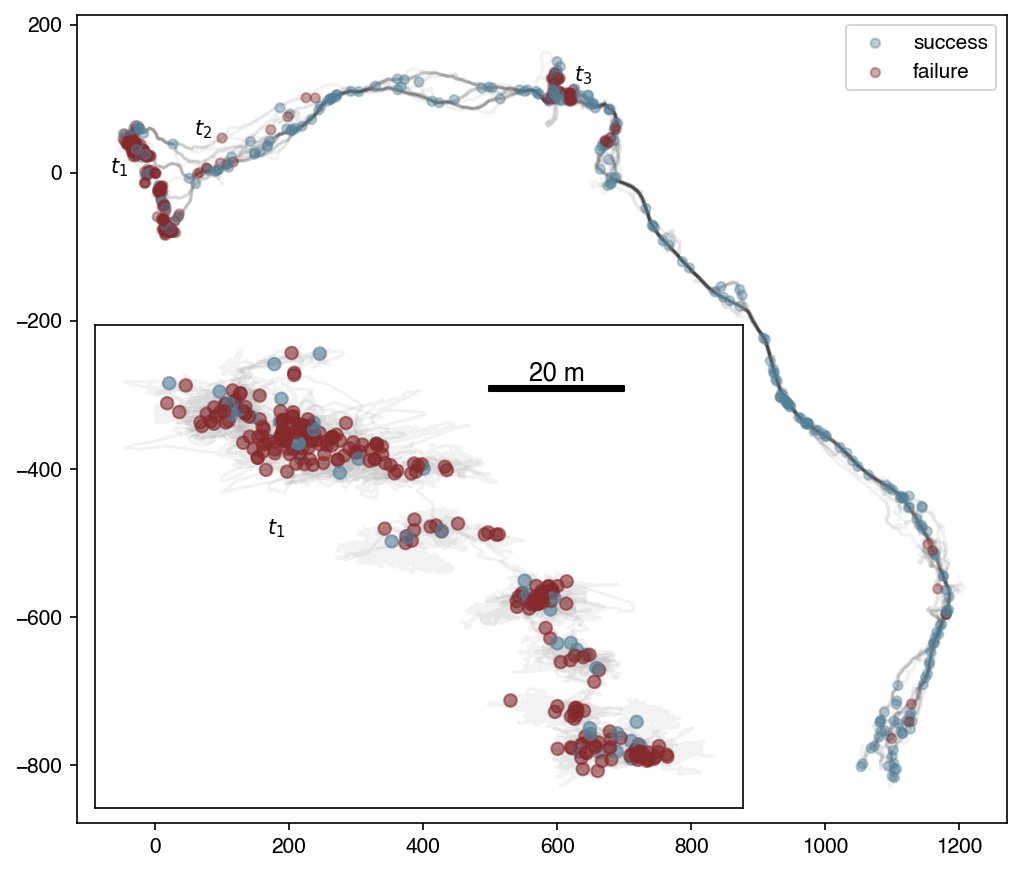
\includegraphics[width=.7\textwidth, valign=t]{../figures/initlocs_1.png}
    \caption{The first 4.5 hours of troop movement on day one of the study period with the locations of the successful (blue) and failed (red) movement initiations during the same morning plotted as well. The approximate location of the troop is also marked at 7,500 seconds (t1), 8,000 seconds (t2), and 12,000 seconds (t3). Finally, the inset shows the troop movement and all events for just the first 7,500 seconds (until t1).}\label{fig:initiations}
\end{figure}

It is unlikely that the majority of the initiations during these common, well defined periods of either milling or moving shed any light on troop dynamics. Much more likely they are noise. In cases of troop milling, most detected initiations likely involve a leading baboon who hardly registers the existence of the following baboon it is supposedly trying to persuade. In cases of troop moving, most are probably cases where the following baboon was only ever going to go in the same direction as the supposed leader.

If the issue were only the aggregation across time periods of radically different troop behavior, one could segment trajectories and perform the same analysis now done in aggregate separately by period. But what is really needed is a proper identification of the meaningful decision points in a day. Simply formalizing this notion is difficult and I don't yet have a good idea of how to do so in a way that enables one to pull out a subset of the already identified initiation events. Working with existing initiation events is compelling because it provides a direct link to existing research that can be used to compare results. However, other framings of the problem are worth exploring as well.

One such framing focuses on larger scale decisions that the troop makes on multiple days. For example, it may have already been clear in figure~\ref{fig:alldata} that the baboons have a primary nesting site and on most days they venture out from this site in either the negative or positive ``x" direction. Figure~\ref{fig:lrtraj} makes this pattern more apparent by only visualizing the first 14 days of trajectories until they reach a distance of 1,000 meters from the origin. The question is, on any particular day, what determines whether the troop moves in the negative or positive ``x" direction?

\begin{figure}[H]
    \centering
    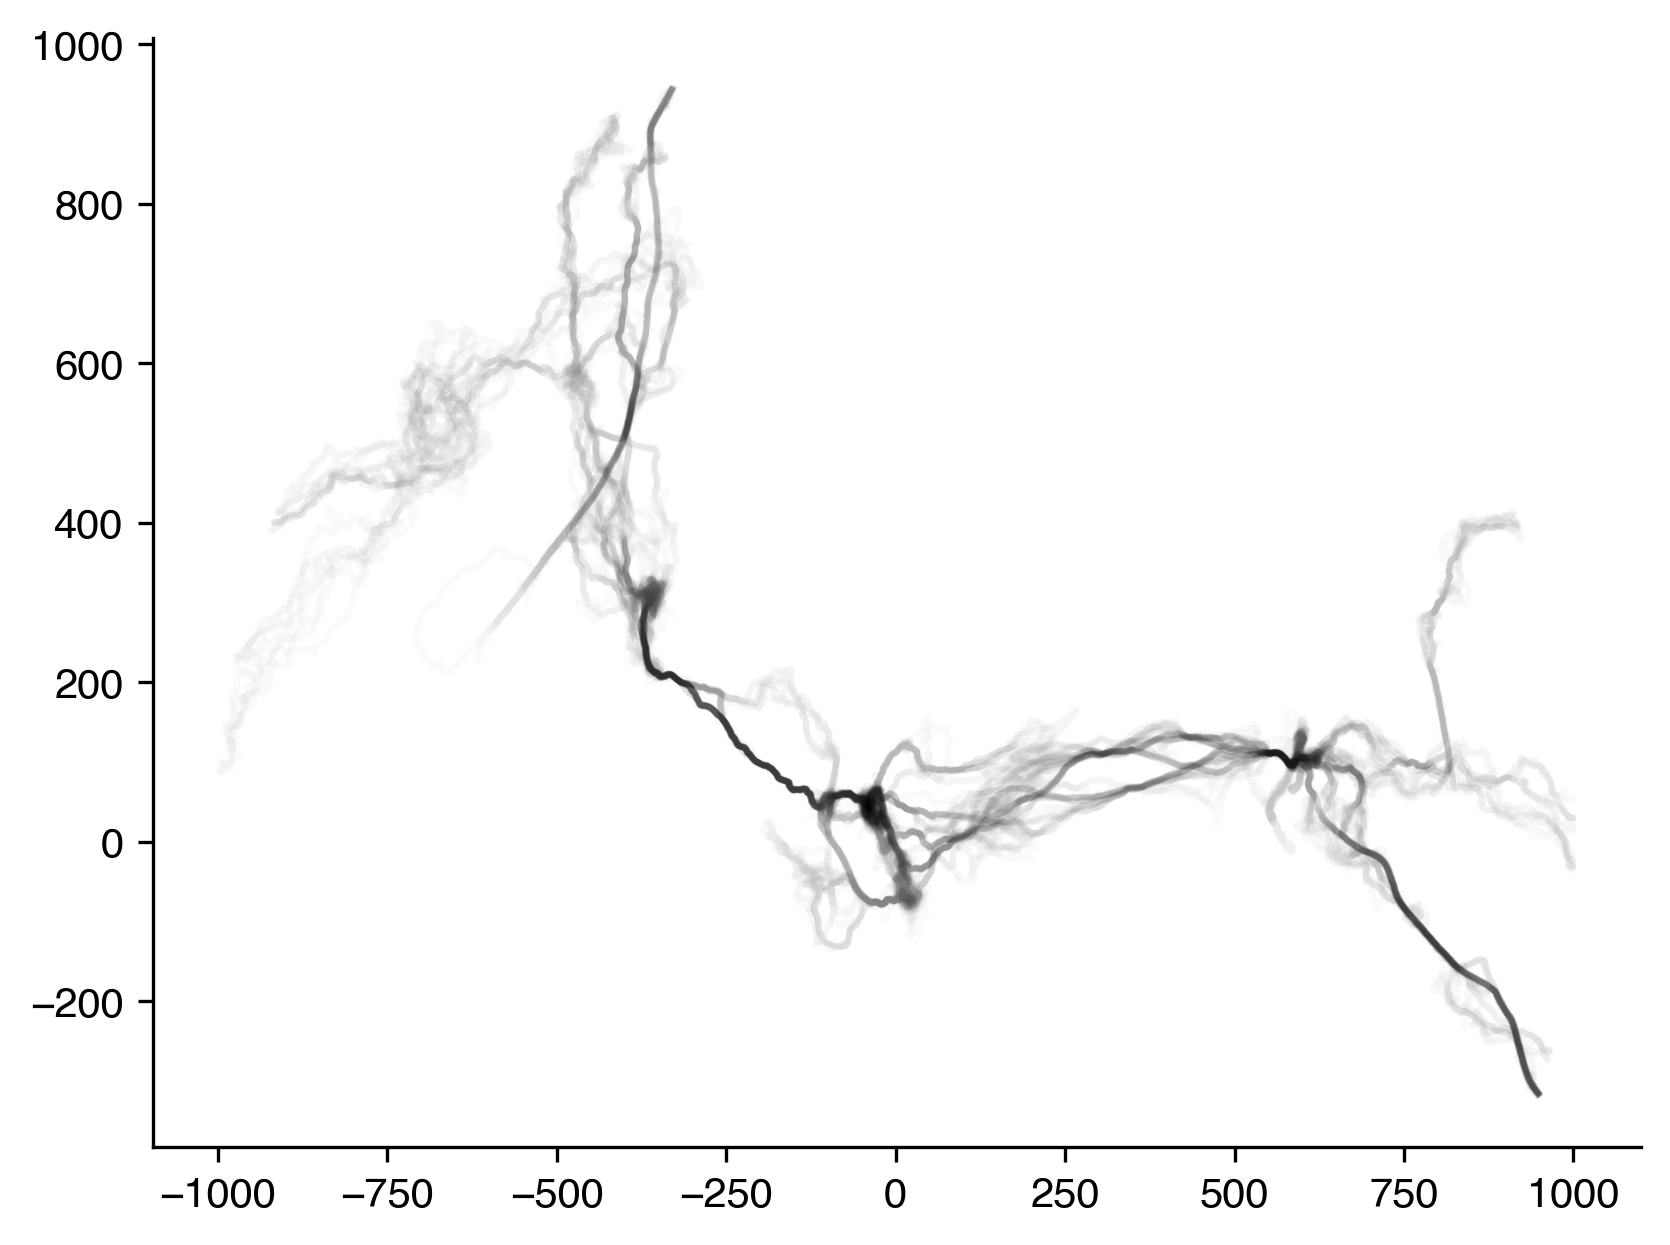
\includegraphics[width=.5\textwidth, valign=t]{../figures/rltrajectories.png}
    \caption{All trajectories from the first 14 days of the study period until they reach a distance of 1,000 meters from the origin. The troop's pattern of movement away from the nesting site near the origin in either the positive or negative ``x" direction is apparent.}\label{fig:lrtraj}
\end{figure}

While I have yet to arrive at a good way to analyze individual baboons in the context of this binary decision, the coarse-graining method discussed above has generated some insights. Figure~\ref{fig:lrprob} shows the probability that a baboon in a particular hexagon ends up going in the positive ``x" direction. The boundaries that appear suggest there may be meaningful locations in space that serve as decision points. If a baboon ventures into such a location it may be a strong signal that this baboon is attempting to pull the group one way or the other. One could imagine these changes in uncertainty serving as the basis for a new movement initiation study. Hopefully, further work visualizing the system will lead to greater clarity on how to analyze this and potentially other large-scale decisions.

\begin{figure}[H]
    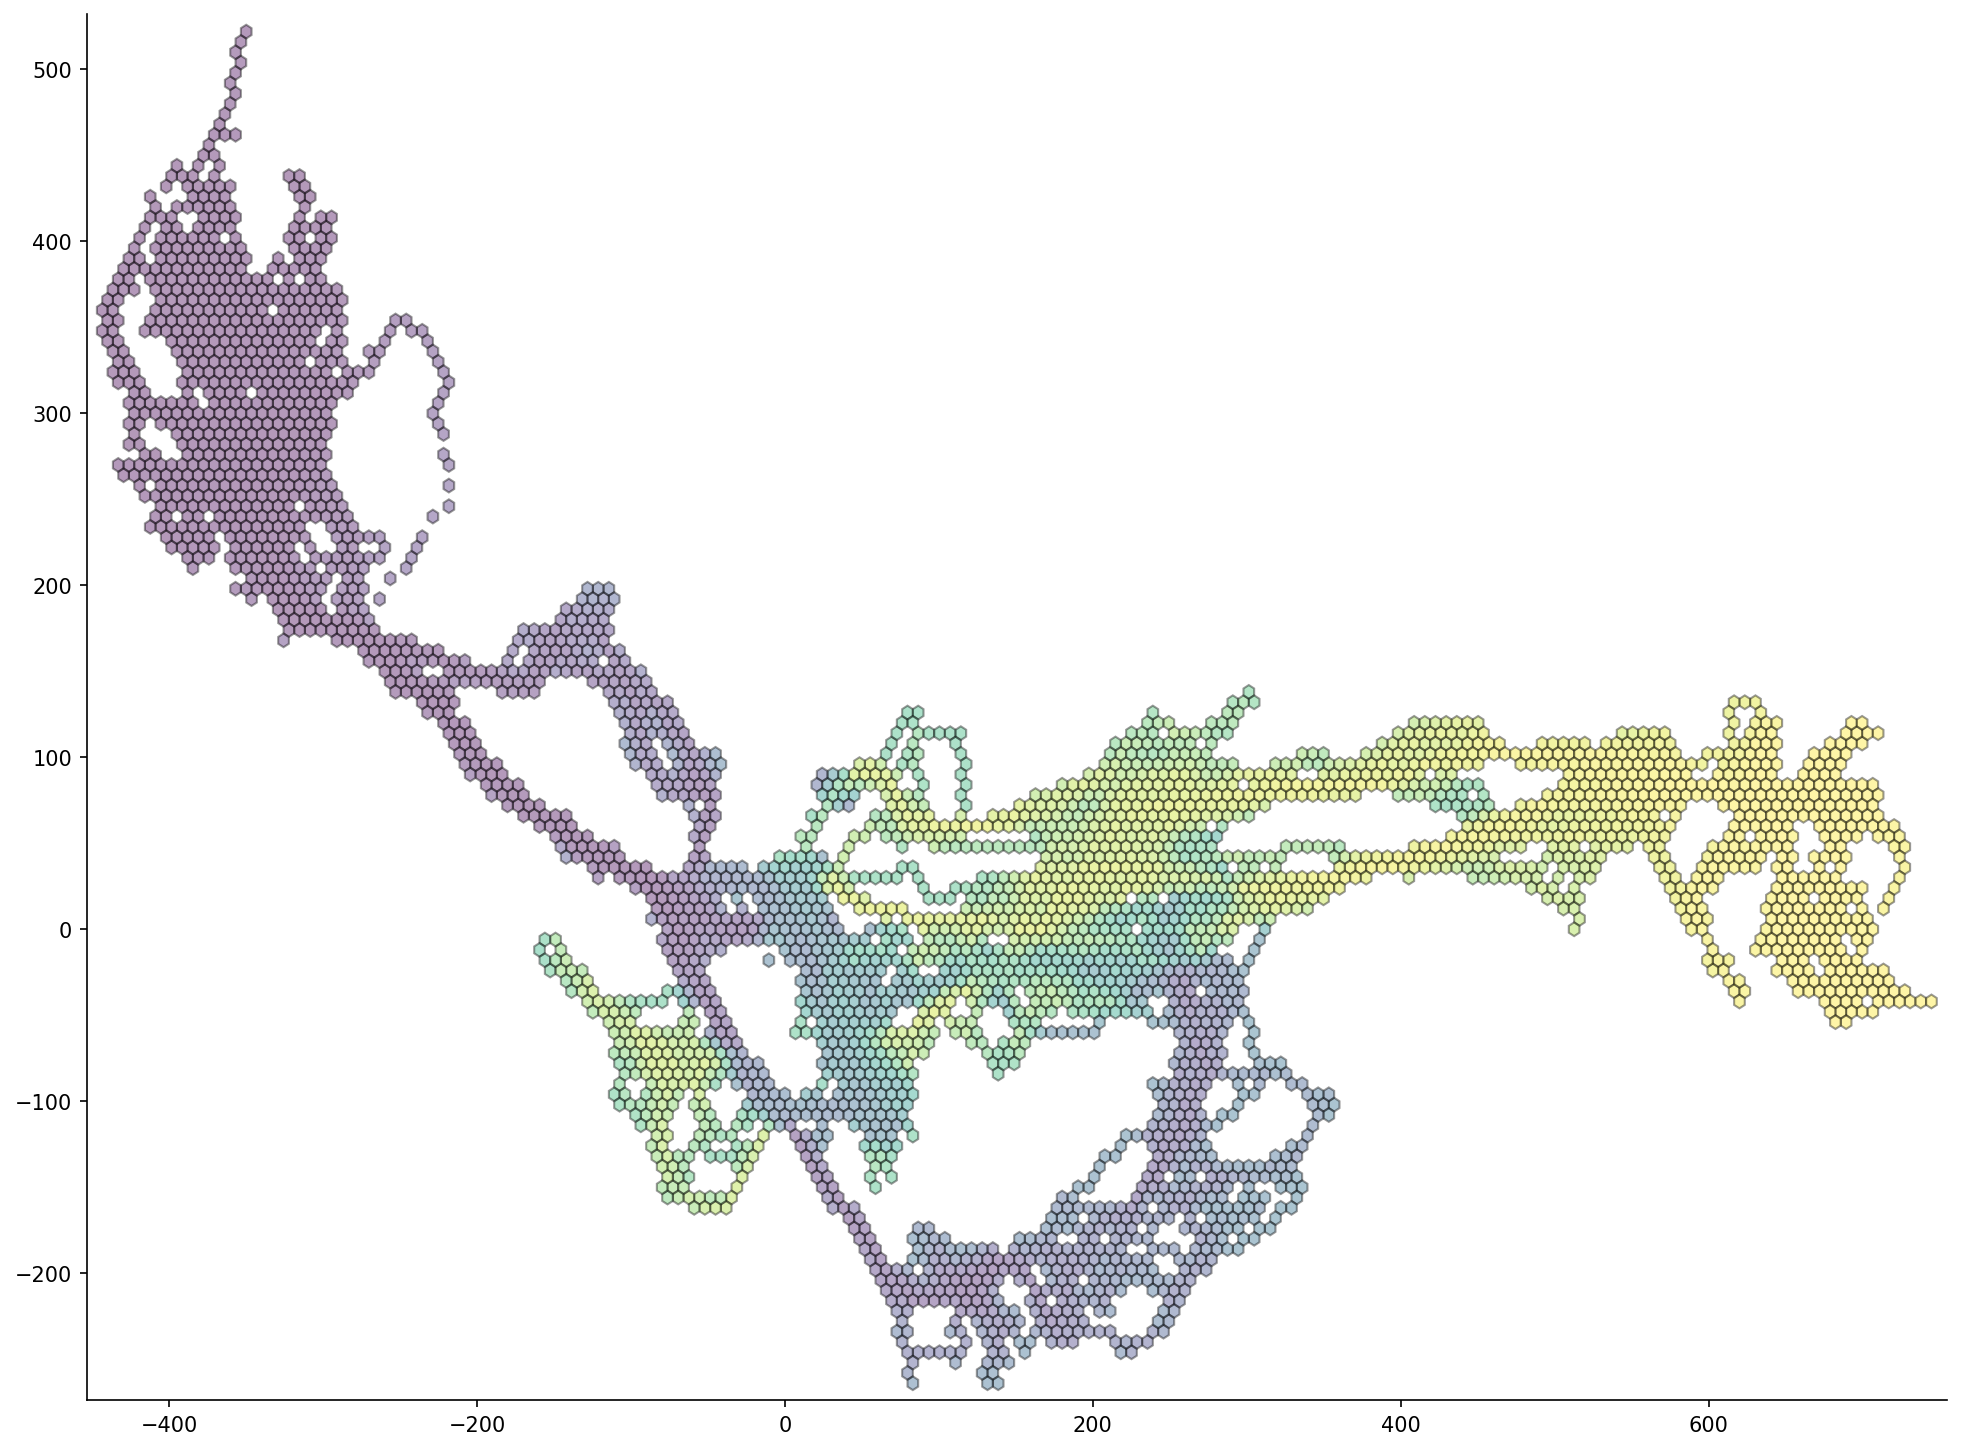
\includegraphics[width=\textwidth, valign=t]{../figures/lrprob.png}
    \caption{A visualization of the probability that a baboon observed at a location ends up going in the positive rather than negative ``x" direction that day. A probability of 1 is represented by the color yellow, 0 by purple, and the rest by blues and greens in between. Since the troop is cohesive, this also represents the probability that the troop goes in the positive ``x" direction conditional on a baboon being seen at a particular location. The places where there is rapid change in color from one hexagon to the next suggest potentially meaningful decision points and thus places for analysis.}\label{fig:lrprob}
\end{figure}

In conclusion, baboons are a fascinating social system and we remain uncertain of the mechanisms driving their decision making with respect to how to forage. I have discussed past research, pointed out its flaws, and hopefully built a compelling case for why a slightly different approach is needed. To support this future work I've produced a coarse-graining scheme that allows for discrete analyses to be conducted and then compared across multiple scales. I'm now looking for the right pairing of question and methodology that can identify meaningful decision points conceptually and empirically. To uncover the leadership dynamics in even a single region or at a particular time of day would be a significant finding.

\bibliographystyle{plain}
\bibliography{refs}

\end{document}
